\section{Unbalanced Tree Search}
Problem definition. Maybe show a partial tree.

Concurrent work-stealing.

Figure~\ref{fig:uts-state} shows the main state transitions.

\begin{figure}
\centering
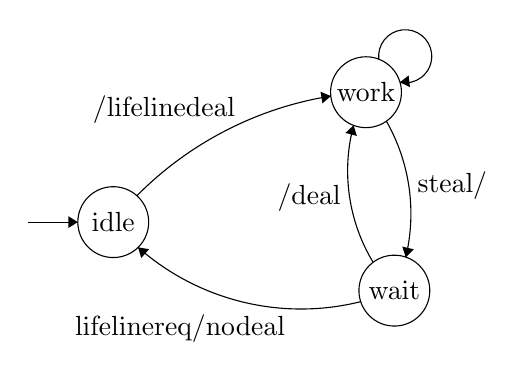
\begin{tikzpicture}[scale=0.15]
\tikzstyle{every node}+=[inner sep=0pt]
\draw [black] (20.9,-23.3) circle (3);
\draw (20.9,-23.3) node {idle};
\draw [black] (42.3,-12.3) circle (3);
\draw (42.3,-12.3) node {work};
\draw [black] (44.7,-29.1) circle (3);
\draw (44.7,-29.1) node {wait};
\draw [black] (22.9,-21.066) arc (135.27934:99.12868:29.75);
\fill [black] (39.32,-12.63) -- (38.45,-12.26) -- (38.61,-13.25);
\draw (25.2,-15.02) node [above] {/lifelinedeal};
\draw [black] (43.382,-9.514) arc (186.50322:-101.49678:2.25);
\fill [black] (45.17,-11.46) -- (46.02,-11.87) -- (45.91,-10.88);
\draw [black] (44.023,-14.75) arc (29.69026:-13.43006:15.827);
\fill [black] (45.67,-26.27) -- (46.34,-25.6) -- (45.37,-25.37);
\draw (46.63,-20.18) node [right] {steal/};
\draw [black] (42.903,-26.704) arc (-148.86241:-194.87738:14.991);
\fill [black] (41.25,-15.1) -- (40.56,-15.75) -- (41.52,-16);
\draw (40.2,-21.24) node [left] {/deal};
\draw [black] (41.852,-30.034) arc (-75.95772:-131.43403:20.846);
\fill [black] (23,-25.44) -- (23.27,-26.34) -- (23.93,-25.59);
\draw (26.55,-31.11) node [below] {lifelinereq/nodeal};
\draw [black] (13.7,-23.3) -- (17.9,-23.3);
\fill [black] (17.9,-23.3) -- (17.1,-22.8) -- (17.1,-23.8);
\end{tikzpicture}
\caption{State diagram for UTS workers.\label{fig:uts-state}}
\end{figure}

Common implementation of WorkList. Show interface. Explain mutability and
ownership are for performance.

Akka: implementation using vanilla actors (no akka-fsm). Work is split up by
sending \lstinline{Work} messages to oneself. State transitions are implemented
using \lstinline{become}.

Termination is difficult.

UTS: three problems, three solutions.

UTS \apgas: concurrency control implemented as multiple paradigms (synchronized
data access, global invariants, active messages). Concurrency is more
fine-grained.
